\documentclass[a4paper, 11pt]{article}
\usepackage[left=3cm, top=3cm, right=2cm, bottom=2cm]{geometry}
%pacote que define as margens
\usepackage{helvet}\renewcommand{\familydefault}{\sfdefault} % define a fonte ARIAL como padrão do texto
\usepackage[utf8]{inputenc} %pacote que permite a utilização de acentos
\usepackage[T1]{fontenc}
\usepackage[brazil]{babel} %pacote que define o idioma
\usepackage{graphicx} %pacote que permite a inserção de imagens
\pagestyle{myheadings} %pacote que define o cabeçalho com o número de página no canto superior direito
\usepackage{setspace} %pacote que permite especificar o espaçamento entre linhas no documento
\usepackage{indentfirst}\setlength{\parindent}{1cm} %pacote que faz indentação na primeira linha do parágrafo
\usepackage{float} %Pacote que permite tabelas flutuarem em qualquer posição
\usepackage[alf,abnt-repeated-title-omit=yes,abnt-emphasize=bf,abnt-etal-list=0]{abntex2cite} %define os parâmetros necessários para as referências e citações de acordo com a ABNT
\usepackage{amsthm} % Pacote que permite a utilização de teoremas
\usepackage{amsfonts} % Pacote que permite a utilização de símbolos matemáticos
\usepackage{caption} % Pacote que permite a inserção de legendas em figuras
\usepackage{subcaption} % Pacote que permite que imagens possam ser inseridas em composições de imagens lado a lado com o \subfigure
\usepackage{amssymb} %4 Pacotes responsáveis pela formatação matemática
\usepackage{rotating} %permite que textos, figuras e tabelas possam ser rotacionados
\usepackage{array}    % permite e vetorização de tabelas
\usepackage{longtable} % permite a elaboração de tabelas complexas
\usepackage{colortbl} % permite a utilização de paletas de cores
\usepackage{tikz} % criação de objetos vetoriais
\usepackage{mathtools} % permite a utilização de equações matemáticas
\usetikzlibrary{shapes, arrows.meta, positioning} % permite a utilização de formas e setas
\usepackage{pdflscape} % permite alterar o estilo da pagina entre portrato e paisagem
\usepackage{sectsty} % permite a alteração do estilo das seções
\sectionfont{\fontsize{12}{12}\selectfont}
\subsectionfont{\fontsize{12}{12}\selectfont}
\subsubsectionfont{\fontsize{12}{12}\selectfont}
\usepackage{url} % permite a utilização de links
\usepackage{pgfplots} % permite a criação de gráficos
%\usepackage{xcolor}
\usepackage[table,xcdraw]{xcolor} % permite a utilização de cores
\usepackage[brazilian,hyperpageref]{backref}    % Paginas com as citações na bibl
\usepackage{hyperref}
\usepackage{polyglossia}
\setmainlanguage{brazil}
%\usepackage{microtype} % para melhorias de justificação
\hypersetup{
    colorlinks=true,
    linkcolor=black, % alterado para black, antes darkblue por bug
    filecolor=magenta,
    urlcolor=blue,
    citecolor=black,
    pdftitle={mybib},
    pdfpagemode=FullScreen
}
%\usepackage[num,overcite]{abntex2cite} % Citações padrão ABNT
%\usepackage{cite}
%\usepackage{pgfgantt}  % gera gantt em latex
\usepackage{acronym}
%\usepackage[acronym]{glossaries} % cria glossário de siglas
%\makeglossaries
\usepackage[most]{tcolorbox}
\usepackage{listings}
\usepackage{cite}
\usepackage{mdwtab}
%\usepackage{mdwtab}
%\usepackage{fancybox}
\lstset{
    inputencoding=utf8,
    extendedchars=true,
    literate={á}{{\'a}}1 {é}{{\'e}}1 {í}{{\'i}}1 {ó}{{\'o}}1 {ú}{{\'u}}1
        {Á}{{\'A}}1 {É}{{\'E}}1 {Í}{{\'I}}1 {Ó}{{\'O}}1 {Ú}{{\'U}}1
        {à}{{\`a}}1 {è}{{\`e}}1 {ì}{{\`i}}1 {ò}{{\`o}}1 {ù}{{\`u}}1
        {À}{{\`A}}1 {È}{{\`E}}1 {Ì}{{\`I}}1 {Ò}{{\`O}}1 {Ù}{{\`U}}1
        {ã}{{\~a}}1 {õ}{{\~o}}1 {Ã}{{\~A}}1 {Õ}{{\~O}}1
        {â}{{\^a}}1 {ê}{{\^e}}1 {î}{{\^i}}1 {ô}{{\^o}}1 {û}{{\^u}}1
        {Â}{{\^A}}1 {Ê}{{\^E}}1 {Î}{{\^I}}1 {Ô}{{\^O}}1 {Û}{{\^U}}1
        {ç}{{\c{c}}}1 {Ç}{{\c{C}}}1
}



\definecolor{codegreen}{rgb}{0,0.6,0}
\definecolor{codegray}{rgb}{0.5,0.5,0.5}
\definecolor{codepurple}{rgb}{0.58,0,0.82}
\definecolor{backcolour}{rgb}{0.95,0.95,0.92}

\lstdefinestyle{mystyle}{
    backgroundcolor=\color{backcolour},
    commentstyle=\color{codegreen},
    keywordstyle=\color{magenta},
    numberstyle=\tiny\color{codegray},
    stringstyle=\color{codepurple},
    basicstyle=\ttfamily\footnotesize,
    breakatwhitespace=false,
    breaklines=true,
    captionpos=b,
    keepspaces=true,
    numbers=left,
    numbersep=5pt,
    showspaces=false,
    showstringspaces=false,
    showtabs=false,
    tabsize=2
}

\lstset{style=mystyle}


\begin{document}
    \thispagestyle{empty}

\begin{center}
	\begin{figure}[h]
  \centering
		
\includegraphics[width=0.21\linewidth]{images/ufpa}
		\label{fig:ufpa}
	\end{figure}


	\vspace{1cm}
	\large \uppercase{UNIVERSIDADE FEDERAL DO PARÁ}\\
	\large \uppercase{INSTITUTO DE TECNOLOGIA}\\
	\vspace{7cm}
	\large \uppercase{TRABALHO: ANÁLISE ESTRUTURAL}\\
	\vspace{1cm}
	\large \uppercase {MATERIA XXX} \\
	\vspace{7cm}
	\large {BELÉM/PA \\ 2025}

 \newpage
 \thispagestyle{empty}
 \large \uppercase{alunos - 0000000000}\\
 \vspace{7cm}

 \singlespacing
 \hspace{8cm} % posicionando a caixa de texto
 \begin{minipage}{7cm}
	Atividade referênte a matéria de resistência dos materiais, entregue para aprovação disciplinar. \\

	Profa. Dr.: Fulano de tal \\
	\vspace{1cm}

	Belém-PA 3 de fevereiro de 2025
	\vspace{4cm}
\end{minipage}

\onehalfspacing
\begin{center}

	EXAMINADOR\\
	\vspace{3cm}
	\rule{10cm}{0.15mm} \\
	Prof. Dr: Fulano de tal\\
	Universidade Federal do Pará - UFPA
\end{center}
\newpage

\begin{center}
	% BLOCO DE TABELAS
	\thispagestyle{empty}
	\listoftables
	\newpage
	% BLOCO DE ABREVIATURAS
	\makeglossaries
    % BLOCO DE FIGURAS
    \thispagestyle{empty}
	\listoffigures
	\newpage
    % SUMARIO
    \thispagestyle{empty}
    \tableofcontents

\end{center}

\newpage
\thispagestyle{empty}

\end{center}
    \section{Apresentação do Trabalho}
\label{sec:apresentacao}


\section{Introdução}
Este trabalho tem como objetivo a análise da envoltória do momento fletor em uma viga isostática sob a ação de uma carga móvel. O estudo inclui a consideração de cargas permanentes e móveis e a determinação dos valores máximos e mínimos do momento fletor ao longo da viga.


\section{Dados para o Trabalho}
Os seguintes valores devem ser adotados:
\begin{table}[h]
    \centering
    \begin{tabular}{|c|c|c|c|c|c|c|}
        \toprule \hline
        \textbf{Equipe} & $c$ (m) & $b$ (cm) & $h$ (cm) & $F_1=F_2$ (kN) & $F_3$ (kN) & $q_{\text{móvel}}$ (kN/m) \\  \hline
        \midrule  \hline
        01              & 2,0     & 30       & 100      & 4,0            & 12,0       & 2,0                       \\  \hline
        \bottomrule
    \end{tabular}
    \caption{Parâmetros para o cálculo da envoltória}
    \label{tab:parametros}
\end{table}


\section{Definições e Parâmetros}

\subsection{Viga Isostática sob a Ação de uma Carga Móvel}
A viga isostática será submetida a um carregamento móvel do tipo trem, além de sua carga permanente correspondente ao peso próprio do concreto armado e de esforços pontuais.

\subsection{Carga Permanente}
A carga permanente é representada pelo peso próprio da viga, considerando uma seção de dimensões $b \times h$ cm$^2$:

\begin{itemize}
    \item base da viga: $b=30cm$ cm;
    \item altura da viga: $h=100cm$ cm.
    \item densidade específica do concreto: $\rho=2000 kg/m^3$
    \item aceleração da gravidade: $g=9,81 m/s^2$
    \item carga permanente: $q_{\text{perm}} = \rho \cdot g \cdot b \cdot h = 5,886 kN/m$ \textdownarrow
    \item Módulo de Elasticidade do Concreto: $E_c = 200 GPa$
    \item Inércia da Seção Transversal: $I = \frac{b \cdot h^3}{12} \rightarrow I = 2.5 \times 10^6 \text{ cm}^4$
    \item Distância entre as forças: $d = 1,5 m$
    \item Comprimento de secção: $c = 2 m$
    \item Número de seções: $n = 11$ (incluindo as extremidades)
\end{itemize}

\begin{figure}[h]
    \centering
    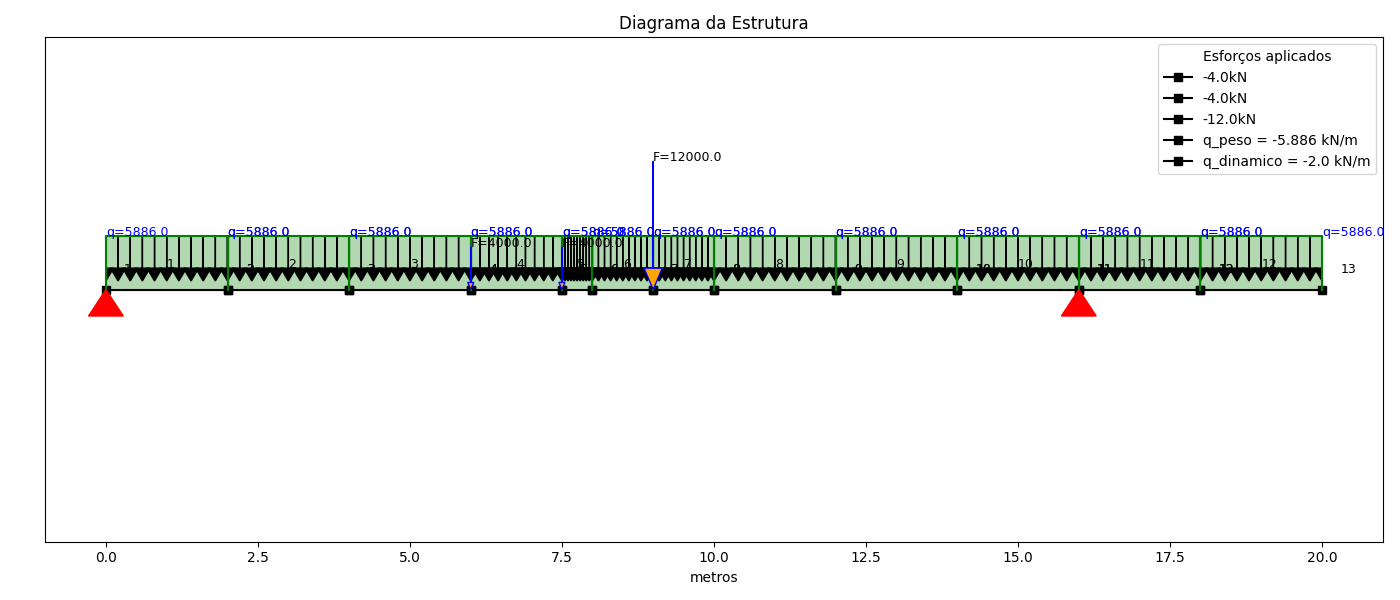
\includegraphics[width=1\linewidth]{images/diagrama}
    \caption{Viga Isostática Simulada}
    \label{fig:viga_isostatica}
\end{figure}

\subsection{Cargas Móveis}
O carregamento móvel é representado por um trem-tipo, com as seguintes características:
\begin{itemize}
    \item carga móvel: $q_{\text{móvel}} = 2 kN/m$ \textdownarrow
    \item Forças pontuais: $F_1 = F_2 = 4 kN$ e $F_3 = 12 kN$ \textdownarrow
    \item comprimento do trem: $L = 1.5 m$
    \item distância entre os trens: $a = 0 m$
    \item número de trens: $n = 3$
\end{itemize}

As três cargas móveis foram distrubidas entre os pontos \textit{S4} e \textit{S6} da viga. Além dos carregamentos pontuais $F_1$, $F_2$ e $F_3$. que também foram distribuídos entre os mesmos pontos.


\section{Memorial de Cálculo}
A viga será dividida em 11 seções, incluindo as extremidades. O cálculo do momento fletor será realizado para cada seção, considerando a carga permanente e móvel. O momento fletor será calculado para as seguintes situações:
O Cálculo se inicia com a identificação dos esforços cortantes e das reações de apoio. A partir daí, é possível determinar o momento fletor em cada seção da viga.

\begin{equation}
    \sum F_y = 0 \Rightarrow R_A + R_B = q_1 \cdot 20 + q_2 \cdot 4 + (P_1 + P_2 + P_3)
\end{equation}

\begin{equation}
    \sum M_A = 0 \Rightarrow R_B \cdot 16 - q_1 \cdot 20 \cdot \frac{20}{2} - q_2 \cdot 4 \cdot \left(\frac{6+10}{2}\right) - P_1 \cdot 6 - P_2 \cdot 7.5 - P_3 \cdot 9 = 0
\end{equation}


\section{Tabela de Cálculo da Envoltória}
A envoltória do momento fletor deve ser calculada conforme a tabela a seguir:
\begin{table}[h]
    \centering
    \begin{tabular}{|c|c|c|c|c|c|}
        \toprule \hline
        \textbf{Seção} & $M_{\text{perm}}$ (kN.m) & $M_{\text{móvel,max}}$ (kN.m) & $M_{\text{móvel,min}}$ (kN.m) & $M_{\text{max}}$ (kN.m) & $M_{\text{min}}$ (kN.m) \\
        \midrule  \hline
        S1             & 0                        & 0                             & 0                             & 0                       & 0                       \\ \hline
        S2             &                          &                               &                               &                         &                         \\ \hline
        S3             &                          &                               &                               &                         &                         \\ \hline
        S4             &                          &                               &                               &                         &                         \\ \hline
        S5             &                          &                               &                               &                         &                         \\ \hline
        S6             &                          &                               &                               &                         &                         \\ \hline
        S7             &                          &                               &                               &                         &                         \\ \hline
        S8             &                          &                               &                               &                         &                         \\ \hline
        S9             &                          &                               &                               &                         &                         \\ \hline
        S10            &                          &                               &                               &                         &                         \\ \hline
        S11            & 0                        & 0                             & 0                             & 0                       & 0                       \\  \hline
        \bottomrule
    \end{tabular}
    \caption{Tabela para o traçado da envoltória}
    \label{tab:envoltoria}
\end{table}


\section{Gráficos da Envoltória}
Para a construção da envoltória, serão traçadas três curvas:
\begin{itemize}
    \item \textbf{Curva 1 (preta)}: Representa os valores da coluna (1) da Tabela \ref{tab:envoltoria}.
    \item \textbf{Curva 2 (vermelha)}: Representa os valores da coluna (4).
    \item \textbf{Curva 3 (azul)}: Representa os valores da coluna (5).
\end{itemize}


\section{Conclusão}
Os resultados obtidos devem ser analisados e discutidos, levando em consideração os efeitos da carga móvel e permanente sobre o comportamento estrutural da viga.


\section{Observações}
\begin{enumerate}
    \item O trabalho deve ser entregue em sala no dia XX/02/25 (terça-feira).
    \item A equipe deve conter até quatro participantes.
    \item Os cálculos devem ser apresentados manuscritos.
    \item Os gráficos devem ser gerados em software gráfico.
    \item O coordenador deve anexar a lista dos participantes e suas respectivas tarefas.
\end{enumerate}


\section{Referências Bibliográficas}
\begin{itemize}
    \item ALMEIDA, Maria Cascão Ferreira de. \textit{Estruturas Isostáticas}. Carga Móvel (Páginas 143 a 164).
\end{itemize}
    \newpage


\section{Dados do Problema}

\subsection{Geometria da Viga}
A viga analisada apresenta os seguintes parâmetros geométricos:
\begin{itemize}
    \item \textbf{Largura} (\( b \)): \(30 \text{ cm} = 0.30 \text{ m}\)
    \item \textbf{Altura} (\( h \)): \(100 \text{ cm} = 1.00 \text{ m}\)
    \item \textbf{Comprimento do trecho analisado}: \( c = 2 \text{ m}\)
\end{itemize}

O momento de inércia da seção transversal é calculado como:

\begin{equation}
    I = \frac{b h^3}{12} = \frac{(0.30)(1.00)^3}{12} = 0.025 \text{ m}^4
\end{equation}

\subsection{Propriedades do Material}
\begin{itemize}
    \item \textbf{Módulo de elasticidade} (\( E \)): \(200 \times 10^9 \text{ Pa}\)
    \item \textbf{Módulo de elasticidade transversal} (\( G \)): \(80 \times 10^9 \text{ Pa}\)
    \item \textbf{Massa específica} (\( \rho \)): \(2000 \text{ kg/m}^3\)
    \item \textbf{Coeficiente de Poisson} (\( v \)): 0.3
\end{itemize}

\subsection{Carregamentos Aplicados}
A viga está sujeita a:
\begin{itemize}
    \item Forças pontuais:
    \[
        F_1 = -4 \times 10^3 \text{ N}, \quad F_2 = -4 \times 10^3 \text{ N}, \quad F_3 = -12 \times 10^3 \text{ N}
    \]
    \item Carga distribuída móvel:
    \[
        q_{\text{móvel}} = -2 \times 10^3 \text{ N/m}
    \]
    \item Carga distribuída do peso próprio:
    \[
        q_{\text{peso}} = -A_{\text{área}} \times \rho \times g = -0.30 \times 1.00 \times 2000 \times 9.81 = -5880 \text{ N/m}
    \]
\end{itemize}


\section{Cálculo das Reações de Apoio}
O equilíbrio de forças na viga é dado por:

\begin{equation}
    \sum F_y = 0 \Rightarrow R_A + R_B + q_{\text{peso}} (L_{\text{spam1}} + L_{\text{spam2}}) + q_{\text{móvel}} (2c) + F_1 + F_2 + F_3 = 0
\end{equation}

\begin{equation}
    \sum F_x = 0 \Rightarrow R_A + R_B =145720 \text{N}
\end{equation}

Já o equilíbrio de momentos em relação ao ponto \( A \) é expresso como:

\begin{equation}
    \sum M_A = 0 \Rightarrow q_{\text{peso}} \frac{20^2}{2} + q_{\text{móvel}} \frac{(10^2 - 6^2)}{2} + F_1 \times 6 + F_2 \times 7.5 + F_3 \times 9 + R_B \times 16 = 0
\end{equation}

Resolvendo o sistema de equações acima, encontramos os valores das reações de apoio:

\begin{equation}
    R_A = 58020 \text{N}, \quad R_B = 87700\text{N}
\end{equation}


\section{Determinação dos Esforços na Viga}

\subsection{Momento Fletor \( M(x) \)}
A função do momento fletor ao longo da viga é descrita pelas equações de macaulay para cada trecho de interesse, no caso:

\begin{equation}
    M(x) =
    \begin{cases}
        R_A x + \frac{q_{\text{peso}}}{2} x^2, & 0 \leq x < 2 \\
        R_A x + \frac{q_{\text{peso}}}{2} x^2, & 2 \leq x < 6 \\
        R_A x + \frac{q_{\text{peso}}}{2} x^2 + \frac{q_{\text{móvel}}}{2} (x - 6)^2 + F_1 (x - 6) + F_2 (x - 7.5), & 6 \leq x < 8 \\
        R_A x + \frac{q_{\text{peso}}}{2} x^2 + \frac{q_{\text{móvel}}}{2} (x - 6)^2 + F_1 (x - 6) + F_2 (x - 7.5) + F_3 (x - 9), & 8 \leq x < 10 \\
        R_A x + \frac{q_{\text{peso}}}{2} x^2 + \frac{q_{\text{móvel}}}{2} (x - 6)^2 + F_1 (x - 6) + F_2 (x - 7.5) + F_3 (x - 9) \\ - \frac{q_{\text{móvel}}}{2} (x - 10)^2, & 10 \leq x < 12\\
        R_A x + \frac{q_{\text{peso}}}{2} x^2 + \frac{q_{\text{móvel}}}{2} (x - 6)^2 + F_1 (x - 6) + F_2 (x - 7.5) + F_3 (x - 9) \\ - \frac{q_{\text{móvel}}}{2} (x - 10)^2, & 12 \leq x < 14\\
        R_A x + \frac{q_{\text{peso}}}{2} x^2 + \frac{q_{\text{móvel}}}{2} (x - 6)^2 + F_1 (x - 6) + F_2 (x - 7.5) + F_3 (x - 9) \\ - \frac{q_{\text{móvel}}}{2} (x - 10)^2, & 12 \leq x < 14\\
        R_A x + \frac{q_{\text{peso}}}{2} x^2 + \frac{q_{\text{móvel}}}{2} (x - 6)^2 + F_1 (x - 6) + F_2 (x - 7.5) + F_3 (x - 9) \\ - \frac{q_{\text{móvel}}}{2} (x - 10)^2 + R_B (x-16), & 14 \leq x < 16\\
        R_A x + \frac{q_{\text{peso}}}{2} x^2 + \frac{q_{\text{móvel}}}{2} (x - 6)^2 + F_1 (x - 6) + F_2 (x - 7.5) + F_3 (x - 9) \\ - \frac{q_{\text{móvel}}}{2} (x - 10)^2 + R_B (x-16), & 16 \leq x \leq 20\\
    \end{cases}
\end{equation}

\subsection{Força Cortante \( V(x) \)}
O esforço cortante é obtida pela derivada do momento fletor:

\begin{equation}
    V(x) = -\frac{dM}{dx}
\end{equation}

\subsection{Inclinação \( \theta(x) \)}
O ângulo de inclinação é calculado por:

\begin{equation}
    \theta(x) = \int \frac{M(x)}{E I} dx
\end{equation}

\subsection{Deflexão Vertical \( y(x) \)}
A equação de deflexão da viga é obtida integrando o ângulo de inclinação:

\begin{equation}
    y(x) = \int \theta(x) dx
\end{equation}

\subsection{Condições de contorno para cada secção}

\begin{table}[h]
    \centering
    \renewcommand{\arraystretch}{1.5}
    \setlength{\arrayrulewidth}{0.5mm}
    \setlength{\tabcolsep}{8pt}
    \arrayrulecolor{black}
    \rowcolors{2}{gray!20}{white}
    \caption{\textbf{\normalsize 📌 Resumo das Condições Atualizadas}}
    \label{tab:resumo_condicoes}
    \begin{tabular}{>{$}l<{$} | >{$}l<{$} | >{$}l<{$}}
        \toprule \rowcolor{gray!50} \hline
        \textbf{Ponto}                                & \textbf{Esforço Cortante $V(x)$} & \textbf{Momento Fletor $M(x)$} \\
        \midrule\hline
        x = 0m \text{ (apoio simples)}                & V(0) = R_A                       & M(0) = 0                       \\\hline
        x = 6m \text{ (carga pontual } P_1 \text{)}   & V(6^+) = V(6^-) - P_1            & M(6^-) = M(6^+)                \\\hline
        x = 7.5m \text{ (carga pontual } P_2 \text{)} & V(7.5^+) = V(7.5^-) - P_2        & M(7.5^-) = M(7.5^+)            \\\hline
        x = 9m \text{ (carga pontual } P_3 \text{)}   & V(9^+) = V(9^-) - P_3            & M(9^-) = M(9^+)                \\\hline
        x = 16m \text{ (apoio simples)}               & V(16^+) = V(16^-) - R_B          & M(16) = 0                      \\\hline
        \bottomrule
    \end{tabular}
\end{table}

\subsection{Resultados obtidos}
\newpage
\thispagestyle{empty}
\begin{landscape}
    \include{out/nos}
\end{landscape}


\section{Resultados e Gráficos}
Os gráficos a seguir representam os diagramas estruturais da viga:

\begin{figure}[H]
    \centering
    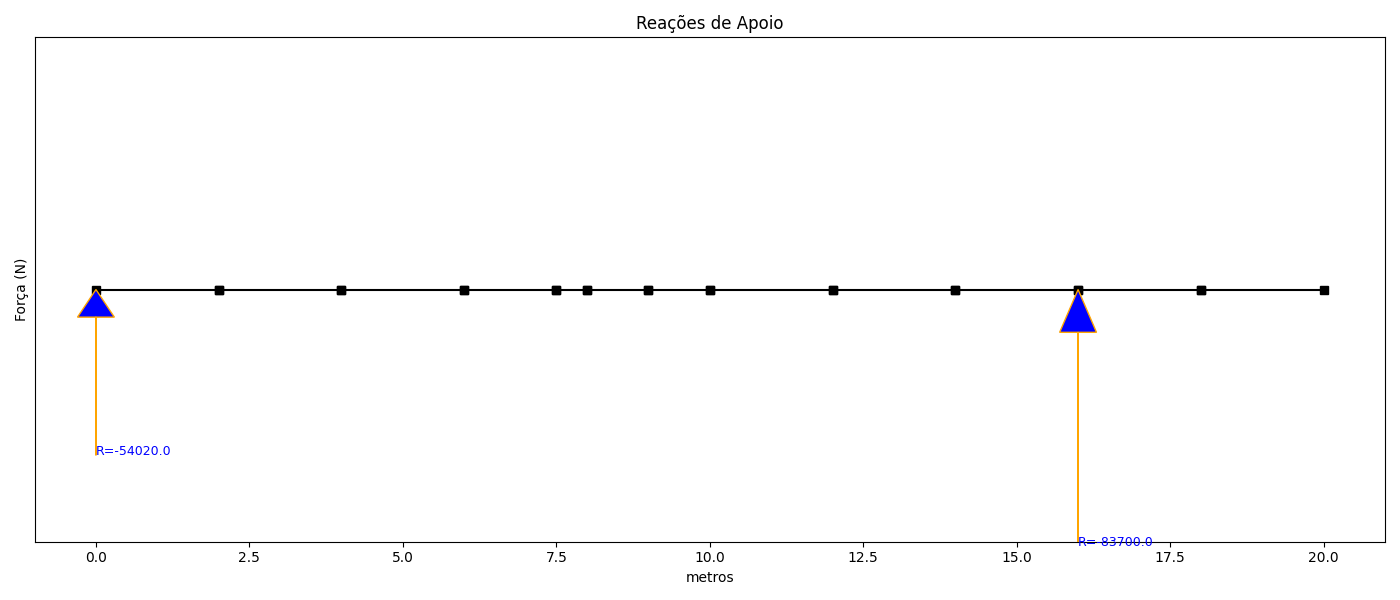
\includegraphics[width=1\textwidth]{images/reacoes}
    \caption{Reações de Apoio}
\end{figure}

\begin{figure}[H]
    \centering
    
\includegraphics[width=1\textwidth]{images/momento}
    \caption{Diagrama de Momento Fletor}
\end{figure}

\begin{figure}[H]
    \centering
    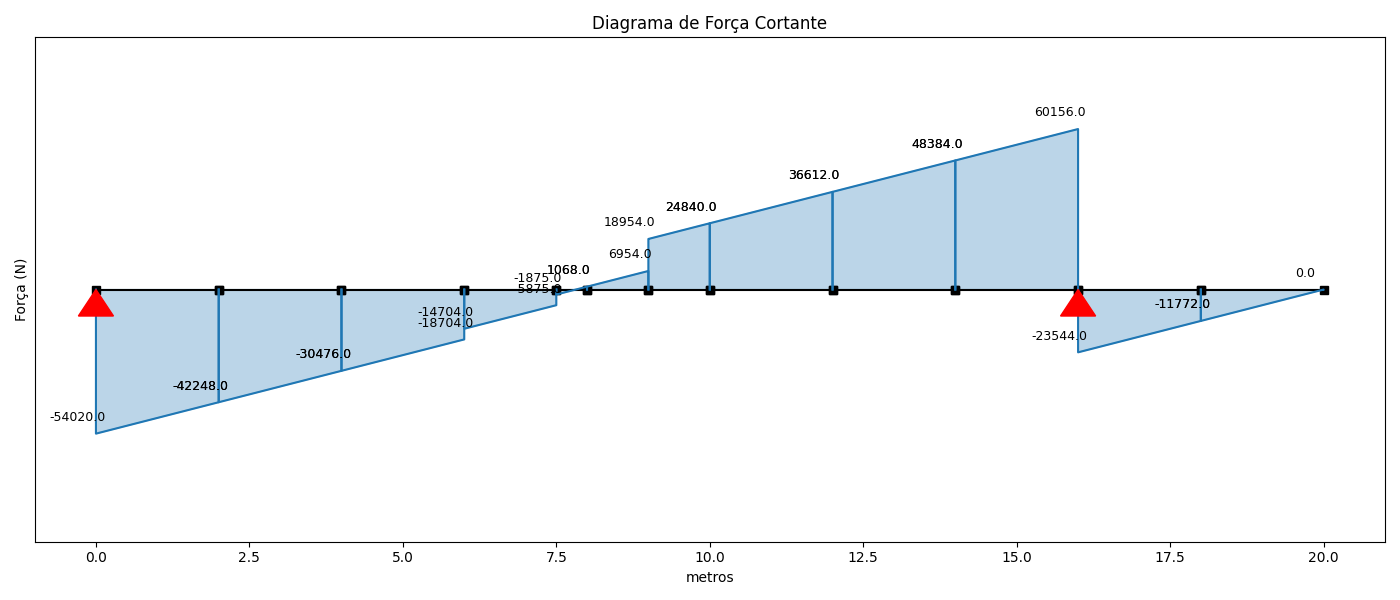
\includegraphics[width=1\textwidth]{images/cortante}
    \caption{Diagrama de Força Cortante}
\end{figure}

\begin{figure}[H]
    \centering
    
\includegraphics[width=1\textwidth]{images/deslocamento}
    \caption{Deformação da Viga}
\end{figure}


\section{Conclusão}
A análise estrutural revelou as distribuições de momento fletor, força cortante e deslocamento ao longo da viga. O método simbólico utilizando Python permitiu calcular as equações dos esforços, garantindo precisão nos resultados.

%    \input{docs/2-1_chip}
%    \input{docs/3_metodologia}
%    \input{docs/3-1_modulos}
%    \input{docs/4_resultados}
%    \input{docs/5_conclusao}
    \bibliographystyle{abntex2-alf}
    \newpage
    \bibliography{docs/bibliography}
\end{document}